% the other packages
\usepackage{amsmath}
\usepackage{amsfonts}
\usepackage{amscd}
\usepackage{amssymb}
% \usepackage{amsthm}
\usepackage{mathrsfs}
\usepackage{bbm}
\usepackage[dvipdfmx]{graphicx}
\usepackage{color}
\usepackage{here}
\usepackage{authblk}

% math def
\newcommand{\argmax}{\mathop{\rm arg~max}\limits}
\newcommand{\argmin}{\mathop{\rm arg~min}\limits}
\newcommand{\bvec}[1]{\mbox{\boldmath $#1$}}
\def\RR{\mathbb{R}}
\usepackage{color}


\makeatletter
\newcommand\appendix@section[1]{%
  \refstepcounter{section}%
  \orig@section*{Appendix \@Alph\c@section: #1}%
  \addcontentsline{toc}{section}{Appendix \@Alph\c@section: #1}%
}
\let\orig@section\section
\g@addto@macro\appendix{\let\section\appendix@section}
\makeatother


% class 4, 9
\newsavebox{\cnine}
\newsavebox{\sfour}
\newsavebox{\sfoursmall}
\newsavebox{\pninethird}
\savebox{\cnine}{
  
\includegraphics[width=0.48cm]{./fig/class_9.pdf}
}
\savebox{\sfour}{
  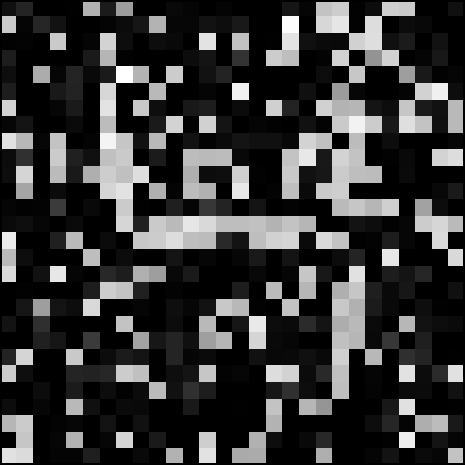
\includegraphics[width=0.48cm]{./fig/sample_4.pdf}
}
\savebox{\pninethird}{
  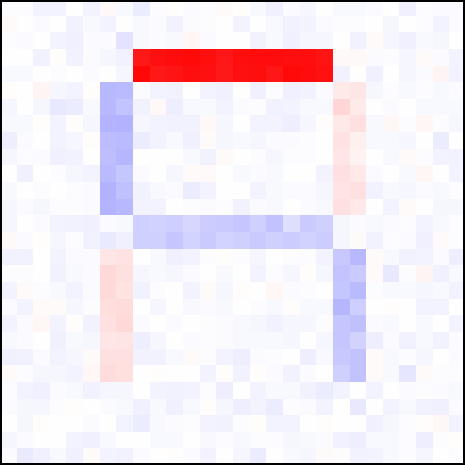
\includegraphics[width=0.48cm]{./fig/3rd_psm_of_9.pdf}
}
\newlength{\bwcnine}
\settowidth{\bwcnine}{\usebox{\cnine}}
\newlength{\bwsfour}
\settowidth{\bwsfour}{\usebox{\sfour}}
\newlength{\bwpninethird}
\settowidth{\bwpninethird}{\usebox{\pninethird}}
%
